% Document settings

% Common
\DocumentMetadata{pdfversion=1.7, pdfstandard=A-2u}
\documentclass[11pt,letterpaper]{article}
\usepackage{fancyhdr}
\usepackage[]{fncychap}
\usepackage{etoolbox} % patch stuff
\usepackage[margin=1in]{geometry}
\usepackage{multirow}
\usepackage{longtable,booktabs, array, threeparttable} % typesetting
\usepackage{bookmark}
\usepackage[acronym]{glossaries-extra}
\pagestyle{plain}
\usepackage{parskip, setspace}

% Plots and Color
\usepackage{graphicx}
\graphicspath{{images/}{drawings/}}
\usepackage[font=footnotesize,labelfont=bf]{caption}
\usepackage{xcolor,colorspace}
\usepackage{tcolorbox}
\usepackage{pgfplots}
\pgfplotsset{compat=newest}
\usepackage{epstopdf}
\usepackage[american voltages]{circuitikz}


% Math stuff
\usepackage{mathtools} % loads amsmath and fixes its bugs, empheq, etc
\usepackage{amssymb}
\usepackage{sympytex}
\usepackage{siunitx}
\sisetup{detect-all=true}   % ensure proper font weight
\DeclareSIPrefix\micro{\ensuremath{\symup{\mu}}}{-6} % ensure upright mu for micro
\sisetup{per-mode = repeated-symbol}    % ensure "/" unit delineator
\sisetup{range-phrase = {\text{~to~}}}  % SI range clarity (NIST 811 Ch7.7)
\DeclareMathSymbol{\varOmega}{\mathalpha}{operators}{"0A}   % upright omega for ohms
\providecommand*{\upOmega}{\varOmega}   % upright Ohms
\DeclareSIUnit{\sq}{\ensuremath{\Box}}    % sheet resistance
\DeclareSIUnit{\Siemens}{S}
\DeclareSIUnit{\torr}{Torr} % add torr to siunitix 3
\DeclareSIUnit\sig{\ensuremath{\sigma}}
\DeclareSIUnit\ppm{ppm}
\usepackage{nicefrac}

% Font
\usepackage{fontspec}
\setmainfont{STIXTwoText}[
	Extension		= .otf,
	UprightFont		= *-Medium,
	BoldFont		= *-Bold.otf,
	ItalicFont		= *-MediumItalic.otf,
	BoldItalicFont 	= *-BoldItalic.otf
]
\usepackage[warnings-off={mathtools-colon,mathtools-overbracket},math-style=ISO]{unicode-math}
\setmathfont{STIXTwoMath-Regular.otf} % for symbols
% \usepackage{microtype}
% \UseMicrotypeSet[protrusion]{basicmath} % disable protrusion for tt fonts
\urlstyle{same}

\usepackage[normalem]{ulem} % Enable normal \ul underline
\usepackage{fancyvrb}

\RequirePackage[type={CC},modifier={by-nc-nd},version={4.0},lang={english}]{doclicense}

\usepackage{datetime2} % to satisfy the "\today" in \hypersetup
\DTMusemodule{english}{en-US}
\usepackage{hyperref}
\hypersetup{
    hyperindex=true,
    colorlinks=true,
	bookmarksnumbered,
    bookmarksopen=true,
    linkcolor=blue,
    filecolor=magenta,      
    urlcolor=cyan,
%%%%%%%%%%%%%%%% METADATA %%%%%%%%%%%%%%%%%%%%	
    pdftitle={EE726 Project 4},
	pdfsubject={8-Bit StrongARM Charge-Redistribution SAR ADC},
    pdfauthor={Chris Biancone},
	pdfpublisher={Chris Biancone},
	pdfkeywords={rail-to-rail; StrongARM; SAR ADC; charge redistribution},
%%%%%%%%%%%%%%%%%%%%%%%%%%%%%%%%%%%%%%%%%%%%%%
	pdfproducer=luaLaTeX-1.18.0,
	pdfdate=\today,
	pdflang={en},pdfmetalang={en},
	pdflicenseurl={},
    % pdfpagemode=FullScreen,
}
\usepackage[noabbrev,capitalize]{cleveref}
% this is necessary for IEEEtranDOI.bst to work with hyperkinked DOIs
\newcommand*{\doi}{}
\makeatletter
\newcommand{\doi@}[1]{\href{https://doi.org/#1}{#1}}
\DeclareRobustCommand{\doi}{\hyper@normalise\doi@}
\makeatother

% % % % % % % % % % % Header footer
% % % % % % % % % % %EDIT THIS % % % % % % % % % % % % % % % % % % % %
\pagestyle{fancy}
\fancyhf{}
\lhead{Tech Memo:  Project 4}
\rhead{Chris Biancone}
\lfoot{EE726}
\cfoot{\today }
\rfoot{Page \thepage}
% % % % % % % % % % % % % % % % % % % % % % % % % % % % % % % % % % % % %

% Scale images if necessary, so that they will not overflow the page
% margins by default, and it is still possible to overwrite the defaults
% using explicit options in \includegraphics[width, height, ...]{}
%\setkeys{Gin}{width=\maxwidth,height=\maxheight,keepaspectratio}

% No paragraph indent
\setlength\parindent{0pt}

\begin{document}

\VerbatimFootnotes % allows verbatim text in footnotes

\numberwithin{equation}{subsection}
\numberwithin{figure}{subsection}

	\hspace{4.5in}
	\includegraphics[width=2in,trim=0cm 0in 0in 0.0in,clip]{images/COE_EME_1505C_hor_k1.pdf}
\newline

\Huge\textbf{EEEE 726: Project 4 \\8-Bit StrongARM Charge-Redistribution SAR ADC}\\

\Large
\textbf{From:} Chris Biancone \\
\textbf{To: } Dr. Mark Pude \\
\textbf{Date: } \today \\
\textbf{Subject: } Project 4\\
\vspace{0.5in}

\section*{Abstract}
\normalsize
This report presents an 8-bit SAR ADC design using the charge redistribution topology and a dynamic StrongArm comparator for low-power operation at a target operating frequency of \qty{1}{Msps} while driving a load capacitance of \qty{1}{\pF}. Control signals are provided by a Verilog control block and the design is verified with AMS simulation in Cadence Virtuoso using the Cadence gpdk045\_v5.0. The ADC achieves <\qty{250}{mLSB} DNL and INL across 45 PVT corners, limited by the number of samples for histogram analysis due to simulation time. 

\section{Design}

This SAR ADC is constructed to meet the requirements specified in \cref{tab:design_req}. Since the comparator is dynamic, the reference current is not used. A typical temperature corner of \qty{40}{\degree\C} is assumed --- simulations at \qty{27}{\degree\C} are not run for this design due to simulation time, since the temperature experienced within an IC would most often be warmer.

\begin{table}[ht]
    \centering
    \begin{tabular}{ccccc}
    \toprule
        \textbf{Specification} & \textbf{Value} & \textbf{Units} & \textbf{Comment} \\
    \midrule
        \(\mathrm{V_{Supply}}\) & 2 \(\pm\)10\% & V & \\
        \(\mathrm{V_{Ref}}\) & 1 & V & \& \qty{2}{\V} RTR\\
        \(\mathrm{I_{Bias}}\) & 10 & \qty{}{\uA} & Not Used \\
        Operating Temp. & \SIrange{0}{85}{} & \qty{}{\degree\C} & Nominal @ \qty{40}{\degree\C} \\
        Sample Rate & 1 & Msps & Clock: \qty{12}{\MHz} \\
        \(N\) & 8 & bits & \\
        \(\mathrm{C_{Load}}\) & 1 & \qty{}{\pF} & Digital Outputs \\
        DNL & \(\pm\)0.5 & LSB & \\
        INL & \(\pm\)1 & LSB & \\
        \(\mathrm{I_{Total}}\) & --- & A & Report \\
        Floorplan Area & --- & \qty{}{\um\squared} & Report \\
    \bottomrule
    \end{tabular}
    \caption{Design specifications for SAR ADC.}\label{tab:design_req}
\end{table}

\subsection{Theory of Operation}

Successive Approximation Register (SAR) ADCs represent a clever iteration over topologies like the integrating and flash ADCs by adapting the binary search algorithm to strike a balance between conversion speed and power/layout efficiency, and as such have become the ``workhorse'' ADC for much of the data converter industry. Their topology is also ideal for pipelining, which greatly extends the conversion throughput of the architecture. With every clock cycle, the binary search algorithm compares a reference voltage generated by a DAC in the middle of the conversion range with the input voltage, determines if it is higher or lower than the input, and subsequently adjusts the reference to the middle of the new range where the input must be. This process is repeated until the bit depth of the ADC is exhausted. While traditionally consisting of sample and hold, comparator, SAR logic, control logic, and DAC blocks, the charge-redistribution SAR ADC subsumes the SAR logic and DAC functionality into a single capacitor array, often following some form of binary encoding based on the chosen switching procedure. Aside from decreasing the total number of circuit elements necessary to construct the ADC, relying on the principle of charge redistribution provides considerable power savings over combinational logic by relying only on switching. 

For the charge-redistribution design using a single supply, during the sample phase, the top plates of the capacitors are connected to the input voltage on the \(V_{bus}\) node, accumulating a charge \(Q_{total} = 2^N C \cdot V_{in}\), while the node at the negative capacitor plates and attached to the comparator's negative input \(V_x\) is connected to \(V_{ref}\). During the hold phase, \(V_x\) disconnects from \(V_{ref}\), the \(V_{bus}\) node is reattached to \(V_{ref}\) and the binary capacitor array and ``dummy'' unit capacitor top plates are switched to \(VSS\). This essentially flips the voltage on the capacitors with respect to the charge accumulated from the input. From here, the bits are cycled by attaching the top plates of the capacitors one by one to the \(V_{bus}\) line that is attached to \(V_{ref}\) in order from MSB to LSB. Since \(V_x\) is only connected to the comparator input, the general case for the voltage at the comparator input with no offset is shown in \cref{eq:vx}.

\begin{equation}
    V_x = \frac{\alpha}{2^N}V_{ref} - V_{in} \quad, \quad \alpha = \left\lfloor 2^N \cdot \frac{V_{in}}{V_{ref}} \right\rfloor \label{eq:vx}
\end{equation}

The switching continues while recording the comparator output for each bit's value. The functionality of this system can be thought of as a closed-loop feedback system where \(V_x\) approaches \(V_{in}\) in quantized steps.

\subsection{Capacitors}

Since the design of this ADC requires precise control of capacitor values, mismatch must be factored into the design considerations. While one can be overly pessimistic and assume a worst-case mismatch of \(+\Delta C\) on the MSB capacitor and \(-\Delta C\) elsewhere, this does result in considerable overdesign and may lead to slower performance than is necessary to meet yield. Since capacitors can very similarly to MOSFETs (dependent on the type), a simple application of Pelgrom's theorem of device sizing shows that the overall variance contribution decreases in a square root fashion as size increases. While there is no closed form solution for the full random variable analysis, a simple approximation shown in \cref{eq:cap_mc} can be used for this design with \(2^N\) capacitors.

\begin{equation}
    \frac{\Delta C}{C} < \frac{1}{2}\frac{\sqrt{2^{N-1}}}{2^N-1} \label{eq:cap_mc}
\end{equation}

Larger capacitors also reduce the impact of any kickback noise generated by the comparator, where current couples through the parasitic capacitances at the comparator inputs and accumulates charge onto the capacitor array. Additionally, \nicefrac{kT}{C} noise is minimized with larger sizing.

However, the capacitors cannot be made infinitely big for speed and layout area considerations. Since the switches used in an IC design have finite resistance when closed, this couples with the capacitor array to create an RC time constant for charging the array. The capacitors and MOSFET switches must be sized in conjunction to ensure that the array will be charged to well-under \qty{1}{LSB} of the actual input voltage in the case of the largest expected voltage difference when the switching occurs, all before the next bit cycle. The addition of a dynamic comparator tightens this requirement, such that this charging must happen before the comparator is set to evaluate its inputs. 

This design uses only the MIM capacitors provided by the Cadence gpdk045, as initial simulations using a combination of MIM and MOS capacitors yielded terrible results due to the parasitic resistance associated with the MOS caps. The clock frequency of \qty{12}{\MHz} gives freedom to use relatively large capacitors for resilience against kickback and other noise sources.

\subsection{Charge Injection \& Bootstrapping}

In addition to the comparator kickback as a source of charge injection that can cause voltage error, the switches must also be considered for their ability to dump charge accumulated in the inverted channel back into the capacitor array. To alleviate this issue to some extent at the capacitor array, transmission gates are used as shown in \cref{fig:tg} so that both electrons and holes are injected from the NMOS and PMOS devices, respectively, and cancel each other out to some degree before accumulating in the capacitor. In the critical operations of switching to the input and reference voltages, bootstrapped switches are employed in the presented design to further reduce the injected charge and linearize the on resistance of the switch, which typically increases towards the middle of the common mode range in a traditional T-gate. The bootstrapped switches use a complementary design akin to a T-gate, shown in \cref{fig:boot}. This design is chosen for its simplicity and the overall reduced resistance from using complementary devices.

\begin{figure}[htbp!]
		\centering
		\includegraphics[width=2in]{images/sch_tg.eps}
		\caption{Transmission gate schematic, used to create normally open and normally closed switches alongside an inverter for appropriate clocking.}\label{fig:tg}
\end{figure}

\begin{figure}[htbp!]
		\centering
		\includegraphics[width=4in]{images/sch_bootsw.eps}
		\caption{Bootstrapped switch schematic.}\label{fig:boot}
\end{figure}

The switched capacitor schematic created for this design is done such that each unit capacitor receives its own SPDT switch for connecting to either \(VSS\) for \(V_{bus}\), to provide consistency in the RC constant across the capacitor array and provide equal drive strength to each capacitor.

\subsection{Comparator}

The comparator used in this design is the same rail-to-rail StrongARM comparator used in the previous flash ADC design. The schematic has been updated for simulation purposes to change any device finger definitions to strictly multiplier values for a better approximation of its behavior across monte carlo simulation, as shown in \cref{fig:comp_sch}. Its performance as extracted from layout and simulated at \qty{1.1}{\GHz} is shown in \cref{tab:comp_perf} for reference.

\begin{figure}[htbp!]
		\centering
	    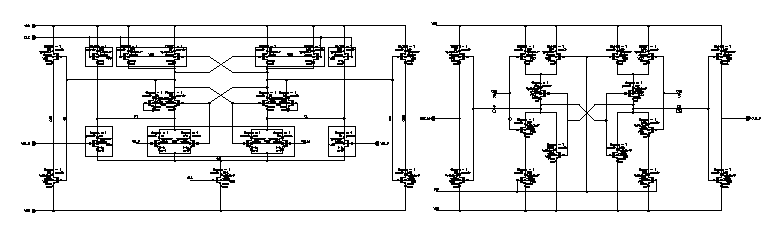
\includegraphics[width=\textwidth]{images/sch_comp_sar.eps}
		\caption{RTR StrongARM comparator schematic with associated SR latch output to avoid invalid outputs.}\label{fig:comp_sch}
\end{figure}

\begin{table}[]
    \centering
    \begin{tabular}{ccc}
    \toprule
        Parameter & Units & Nominal \\
    \midrule
        Hysteresis & mV & 14.64 \\
        Prop. Delay (\qty{1}{\pF}) & ns & 1.5778 \\
        Prop. Delay (\qty{1}{\fF}) & ps & 414.07 \\
        DC Current & nA & 1.2868 \\
        W/decision & pW & 1.067 \\
        Layout Area & \(\qty{}{\um^2}\) & 119.79 \\
    \bottomrule
        
    \end{tabular}
    \caption{Comparator performance with extracted parasitics from layout.}\label{tab:comp_perf}
\end{table}

It is seen in the design of the flash ADC that this comparator design, while having merit for its ability to process a wide range of input signals, the extra devices on the input allow for a lot of kickback noise to be generated. The same kickback reduction scheme is employed in this design, where a transmission gate is placed after the local clock buffer to couple with the parasitic capacitance on the clock line and slow down the charging and discharging of the internal nodes \(V_A\) and \(V_P\), which reduces the current sent back through the inputs through the relationship in \cref{eq:kickback}.

\begin{equation}
    I_{kickback} = -\left(\frac{2}{3}W\,L\,C_{ox} + C_{GS_{tot}}\frac{dV_A(t)}{dt} - C_{GS_{tot}}\frac{dV_P(t)}{dt}\right)\label{eq:kickback}
\end{equation}

Initially, no matter how small the RC time constant was made for charging the capacitor array, the comparator would still evaluate too early and contribute to massive DNL and INL due to its synchronous nature to the switching of the capacitor circuit. Methods of delaying the clock line to the comparator were investigated to hold off its evaluation until the nodes settled, but achieving the amount of delay needed at a clock frequency of only \qty{12}{\MHz} proved difficult without a polyphasic clock or other methods such as a PLL\@. A simple, but rather brute-force, solution was to invert the clock being sent to the comparator, so that it would evaluate half a cycle later and give the capacitors more than enough time to settle. If more time were to be given to this design, it may be desirable to implement a comparator driver within the Verilog controller, with some combinational logic to generate a clock cycle only when the ADC bits are being cycled. This would both increase power savings and reduce the amount of kickback noise generate during the critical sample and hold phase.

\subsection{Encoder}

\section{Schematic Level Simulations}

\subsection{INL and DNL Testbench}

\subsection{Propagation Delay Testbench}

\subsection{Schematic Level Results}

\begin{table}[]
    \centering
    \begin{tabular}{ccccc}
    \toprule
        Parameter & Units & Max & Nominal & Min \\
    \midrule
        DNL & mLSB & 4821.7 & 153.8 & 60.21 \\
        INL & mLSB & 16.009 & 9.2979 & 2.3985 \\
        Max Prop. Delay & ns & 13.253 & 7.4131 & 5.7102 \\
        Timing difference & ps & 213.44 & 148.72 & 18.045 \\
        Reference DC Current & \qty{}{\uA} & 192.95 & 148.72 & 123.55 \\
        Max Transient Current & mA & 15.358 & 8.4772 & 3.502 \\
        W/conversion & pW & 101.38 & 63.452 & 37.654 \\
    \bottomrule
        
    \end{tabular}
    \caption{Flash ADC performance results across PVT corners, with a precision of \qty{10}{mLSB} for DNL and INL measurements.}\label{tab:corners_sch}
\end{table}

\begin{table}[]
    \centering
    \begin{tabular}{ccccc}
    \toprule
        Parameter & Units & Nominal \\
    \midrule
        DNL & mLSB & 115.61 \\
        INL & mLSB & 7.2199 \\
        \(\mathrm{V_{LSB_{eff}}}\) & mV & 66.4 \\
    \bottomrule
        
    \end{tabular}
    \caption{Flash ADC DNL \& INL results at the typical corner, with a precision of \qty{1}{mLSB}.}\label{tab:typ_sch}
\end{table}

\section{Layout Floorplan}

\section{Conclusion}

\newpage

\bibliographystyle{bib/IEEEtranDOI}
\bibliography{bib/export.bib}

\newpage
\section*{Appendix}

\end{document}